\documentclass[11pt]{article}
\usepackage{shared/hanzocover}
\usepackage[utf8]{inputenc}
\usepackage[T1]{fontenc}
\usepackage{amsmath,amssymb}
\usepackage{graphicx}
\usepackage{booktabs}
\usepackage{xcolor}
\usepackage{tikz}
\usetikzlibrary{arrows.meta,positioning,calc}
\usepackage[hidelinks]{hyperref}
\emergencystretch=1.5em

\title{Linkage, Not Similarity:\\
       Context-Sensitive Retrieval for Long-Term Agent Memory}
\author{Zach Kelling\thanks{Corresponding author: research@hanzo.ai} \\
    \textit{Hanzo Industries Inc (Techstars '17)} \\
    Los Angeles, California \\
    \texttt{https://hanzo.ai}}
\date{Revision~1}

\begin{document}

\hanzocoverpage

\twocolumn[
  \begin{@twocolumnfalse}
  \maketitle
  \begin{abstract}
  \noindent
  Vector similarity retrieves what sounds related. Long-term memory has to
  retrieve what is connected: the turn that answers a question is usually
  linked to the turn that matches it by a person, an event or a date, not by
  wording. We measure this on LoCoMo, where a cosine index recovers every
  annotated turn for only \textbf{22.7\%} of multi-hop questions at $k=20$
  while recovering at least one for 80.1\%. A second index of atomic facts,
  each citing the turn it came from, plus two small structural bonuses,
  raises the complete-evidence rate to \textbf{36.2\%} and the any-evidence
  rate to 87.2\% with nothing learned and under a millisecond per query.
  Every term is ablated; the fact index carries most of the gain, and two
  plausible additions---fusion of whole ranked lists and a surface-entity
  hop---make the result worse.

  We then argue that this recall number is a unit test, not a product
  score. LoCoMo question answering is saturating under vendor protocols
  (Mem0 reports 92.5\%, Zep 94.7\%, on protocols that differ from each
  other), and the LoCoMo-Conv benchmark shows that the same memories phrased
  as a user would phrase them expose retrieval gaps the QA form hides. We
  describe the memory record and the read path Hanzo Context uses to close
  those gaps---immutable raw memory; atomic facts with canonical entities and
  validity intervals; query-conditioned planning; bounded typed expansion
  instead of global fusion; a hop whose query is rebuilt from the state the
  previous hop resolved; and deterministic resolution of superseded
  facts---and the protocol on which we evaluate it: a declared dev/test
  split, a frozen commit, LoCoMo, MemoryAgentBench FactConsolidation and
  LoCoMo-Conv, with retrieval and answering reported separately and
  evidence graded EXACT, SUPPORTED or ANSWERED.
  \end{abstract}
  \vspace{1em}
  \end{@twocolumnfalse}
]

\section{The Claim}

A memory system for an agent is asked one thing: given what was said before,
find what bears on what is being asked now. The dominant implementation
embeds every turn, embeds the question, and returns the nearest neighbours.
That works when the answer resembles the question. It fails, quietly, when the
answer is \emph{connected} to the question by something a sentence embedding
does not carry---the same person named two sessions apart, the date a plan
was made and the date it happened, the fact that one turn answers the turn
before it.

This paper makes one technical claim and one methodological one.

The technical claim is that linkage is a separate index, not a better
embedding. Extract short facts from each turn, keep the pointer from every
fact back to the turn it came from, give each fact its entities and its time,
and let a question reach a turn through a fact when it cannot reach it
through the turn's own wording. Section~\ref{sec:locomo} measures this in
isolation: on LoCoMo multi-hop questions the complete-evidence rate at $k=20$
moves from 22.7\% to 36.2\%, and the ablation in Table~\ref{tab:ablation}
attributes most of it to the fact index.

The methodological claim is that the number we just quoted is the wrong one
to optimise. It measures whether every turn an annotator marked was
retrieved. A system can answer correctly from a different turn that says the
same thing; the LoCoMo-Conv authors call this \emph{silent grounding} and
ship extra annotations because strict gold-turn recall misses it
\cite{locomoconv}. Section~\ref{sec:measure} sets out what we measure instead
and why, and Section~\ref{sec:protocol} fixes the protocol before any number
on the test split is read.

\section{What Is Being Measured}
\label{sec:measure}

Three quantities are routinely conflated under ``LoCoMo score''.

\paragraph{Evidence recall.} For each question LoCoMo lists the dialogue
turns that support the answer \cite{locomo}. \textbf{ALL@k} is the fraction
of questions for which every listed turn is in the top $k$; \textbf{ANY@k}
the fraction for which at least one is. The two disagree by a factor of
three on multi-hop questions (Table~\ref{tab:locomo}). ALL is the honest
number for a retriever that must hand a reader complete evidence; ANY is the
honest number for a retriever whose reader can follow a lead.

\paragraph{Answer accuracy.} A reader is given the retrieved turns and
scored on what it says: token-level F1 and exact match against the gold
answer in the LoCoMo paper, or an LLM judge in most vendor reports. This is
what Mem0's 92.5\% \cite{mem0blog} and Zep's 94.7\% \cite{zepresearch} are,
and they are not the same measurement as each other: Zep's page names
gpt-5.4 with medium reasoning as reader and a chain-of-thought gpt-5.4 judge,
median 5,760 context tokens per question, and 1,459 of 1,540 questions
correct; Mem0's post names an April 2026 algorithm, 6.7--7.0K tokens per
retrieval, and states that Zep's figure is disputed by a third-party
re-run at 75.1\%. Neither is comparable to the LoCoMo paper's own F1
figures, and neither is comparable to evidence recall.

\paragraph{Conflict resolution.} MemoryAgentBench's FactConsolidation task
numbers its facts, later facts supersede earlier ones, and the question asks
for the current value, one or two hops deep \cite{mab}. Its metric is
\texttt{substring\_exact\_match}. CAR \cite{car} reports 78.0 / 30.2 on
single- and multi-hop with gpt-4o-mini and 94.8 / 51.5 with gpt-4o, pooled
over context lengths from 6K to 262K tokens; at 262K the same pipelines score
82 / 27 and 93 / 41, against 54 / 5 for HippoRAG-v2 and 60 / 5 for gpt-4o
reading the whole context. Pith's page claims 68.0 exact match on the
262K multi-hop lane \cite{pith}. A comparison circulated in September 2026
placed 91 / 57 beside CAR's pooled numbers without a published method; we
could not locate a stable source for it and do not cite one.

We report each quantity under its own name, never one as another.

\paragraph{Three grades of evidence.} For a question with gold turns $G$ and
retrieved turns $R$, a system scores \textbf{EXACT} if $R \cap G \neq
\emptyset$ (and ALL if $G \subseteq R$), \textbf{SUPPORTED} if some turn in
$R$ shares an atomic fact with a turn in $G$ or contains the gold answer
string, and \textbf{ANSWERED} if the reader's answer is correct. The three
are reported side by side. The gap between EXACT and SUPPORTED is the
annotation's blind spot; the gap between SUPPORTED and ANSWERED is the
reader's.

\section{Related Work}

\paragraph{Benchmarks.} LoCoMo \cite{locomo} provides ten very long
two-person conversations with question--answer pairs and their supporting
turns, in single-hop, multi-hop, temporal, open-domain and adversarial
categories. LongMemEval \cite{longmemeval} tests extraction, multi-session
reasoning, temporal reasoning, knowledge updates and abstention over
scalable chat histories. MemoryAgentBench \cite{mab} recasts long-context
tasks as incremental multi-turn interaction and adds FactConsolidation, the
conflict-resolution task used here. LoCoMo-Conv \cite{locomoconv} rewrites
LoCoMo's memories into dialog, implicit, counterfactual and composed
requests---1,986, 1,986, 1,540 and 1,069 items---and standardises the
memory systems it compares on all-MiniLM-L6-v2 embeddings, $k=10$,
gemma-4-31B-it at temperature 0 as reader, and GPT-5.4-mini with reasoning
as judge, validated against Claude Sonnet 4.5 and Qwen3.6-35B-A3B on a
1,488-item subset. Without rewriting, Recall@10 falls from 0.531--0.659 on
dialog to 0.308--0.456 on implicit queries across five systems.

\paragraph{Systems.} MemGPT \cite{memgpt} manages context as an operating
system manages memory tiers. A-MEM \cite{amem} organises notes Zettelkasten
style. HippoRAG \cite{hipporag} runs personalised PageRank over an extracted
graph. Mem0 \cite{mem0} extracts and consolidates memories, and its 2026
algorithm adds single-pass add-only extraction and entity linking
\cite{mem0blog}. Zep \cite{zep} keeps a temporally aware knowledge graph and
retrieves across facts, entities, episodes, observations and thread
summaries \cite{zepresearch}. AnchorMem \cite{anchormem} extracts atomic
facts as retrieval anchors while preserving the raw context immutably, and
binds related facts into event nodes rather than bridging through generic
entities. AtomMem \cite{atommem} selects high-value atomic facts and
organises them into event structures and temporal profiles. Memora
\cite{memora} indexes a short primary abstraction and several cue anchors
per memory and keeps the full value unindexed, reporting up to 98\% fewer
context tokens. APEX-MEM \cite{apexmem} stores temporally grounded events in
an entity-centric property graph with append-only history and resolves
conflicts at query time, reporting 88.88\% on LoCoMo QA and 86.2\% on
LongMemEval under its setup. Our design takes from each what their own
ablations support: anchors over raw memory, events over entity hops,
abstractions beside cue anchors, append-only temporal history.

\paragraph{Conflict resolution.} CAR \cite{car} separates evidence
extraction from policy: retrieve, extract numbered facts, pick the latest
serial with code, then form the next hop. TEPA \cite{tepa} makes validity an
explicit, revocable state of a memory. MemTxn \cite{memtxn} gives memory a
transaction boundary with source-supported admission and a temporal
resolver. All three converge on the same rule: do not ask the reader which of
two contradicting facts is current.

\section{The Memory Record}
\label{sec:write}

Every write produces one immutable raw memory and a set of derived,
indexed views of it. Nothing derived replaces the raw text; the reader is
always handed the original.

\begin{itemize}
  \item \textbf{raw} --- the turn or document as received, with \textbf{source}
        (conversation, session, turn) and \textbf{observed\_at}.
  \item \textbf{facts[]} --- atomic statements, several per turn, each with a
        canonical \textbf{subject}, a \textbf{relation}, an \textbf{object}
        that is a canonical entity or a literal, an \textbf{event\_time} when
        the text carries one, \textbf{valid\_from} / \textbf{valid\_to} where
        derivable, a \textbf{confidence}, an embedding, and the pointer to
        its source turn.
  \item \textbf{entities[]} --- canonical identifiers resolved by type
        (person, place, organisation, work, date), not by capitalisation. The
        surface heuristic was measured and rejected
        (Section~\ref{sec:negative}).
  \item \textbf{events[]} --- membership of facts in a shared event, the
        associative link AnchorMem found to beat entity bridging.
  \item \textbf{supersedes[] / superseded\_by[]} --- a supersession key so
        that the current value of a relation is a lookup, not a judgement.
  \item \textbf{primary\_abstraction} and \textbf{cue\_anchors[]} --- a short
        phrase saying what the memory is about and several context-aware tags
        that give the same memory alternative entry points.
\end{itemize}

The fact layer is the linkage index. On LoCoMo the dataset's own
observation annotations cite 79.9\% of multi-hop gold turns; the remaining
20\% are unreachable through any fact, which bounds what a re-ranker can do
and is why extraction coverage, measured in Table~\ref{tab:coverage}, comes
before tuning.

\section{The Read Path}
\label{sec:read}

\begin{figure*}[t]
\centering
\resizebox{\textwidth}{!}{%
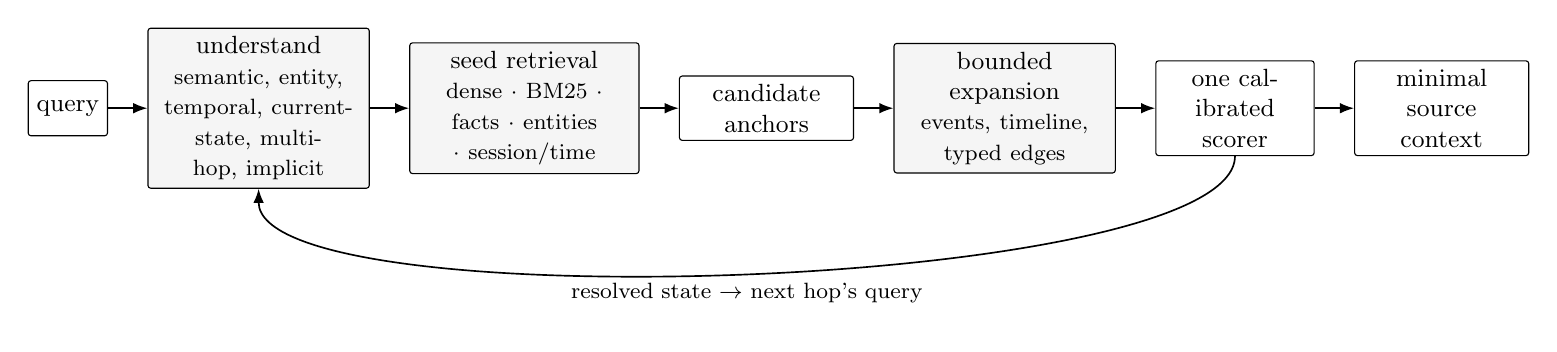
\begin{tikzpicture}[
  node distance=3.5mm and 5mm,
  box/.style={draw, rounded corners=1pt, minimum height=7mm, inner sep=3pt, font=\small, align=center},
  soft/.style={box, fill=black!4},
  arrow/.style={-{Latex[length=1.8mm]}, semithick}
]
\node[box] (q) {query};
\node[soft, right=of q, text width=26mm] (plan) {understand\\ \footnotesize semantic, entity, temporal, current-state, multi-hop, implicit};
\node[soft, right=of plan, text width=27mm] (seed) {seed retrieval\\ \footnotesize dense $\cdot$ BM25 $\cdot$ facts $\cdot$ entities $\cdot$ session/time};
\node[box, right=of seed, text width=20mm] (anch) {candidate\\ anchors};
\node[soft, right=of anch, text width=26mm] (exp) {bounded expansion\\ \footnotesize events, timeline, typed edges};
\node[box, right=of exp, text width=18mm] (score) {one calibrated\\ scorer};
\node[box, right=of score, text width=20mm] (ctx) {minimal\\ source context};
\draw[arrow] (q) -- (plan);
\draw[arrow] (plan) -- (seed);
\draw[arrow] (seed) -- (anch);
\draw[arrow] (anch) -- (exp);
\draw[arrow] (exp) -- (score);
\draw[arrow] (score) -- (ctx);
\draw[arrow] (score.south) to[out=-90,in=-90,looseness=0.35] node[below, font=\footnotesize, midway] {resolved state $\rightarrow$ next hop's query} (plan.south);
\end{tikzpicture}}
\caption{The read path. Every candidate enters through a named generator
and carries the contribution of each term that scored it, so a ranking is
explainable after the fact. A hop that resolves an entity or a date rewrites
the query for the next hop; the original sentence is embedded once and never
reused for hop two.}
\label{fig:read}
\end{figure*}

\subsection{Query understanding}

The question is classified into retrieval operators---semantic, entity,
relationship, temporal, current-value, causal, multi-hop, implicit---by
rules over its surface (a year, a month, a name, ``after'', ``still'',
``most recent'') with a small model consulted only where the rules are
silent. The plan is an explicit state: what is resolved (an entity, a date,
an event), what is unresolved (the relation or object being asked for),
the evidence gathered so far, and the budget in hops, candidates, latency
and context tokens. The weights of the generators below are conditioned on
the plan; a temporal question spends its budget on the timeline, a
current-value question on the supersession chain.

\subsection{Seed retrieval and bounded expansion}

Seeds come from dense search over turns, BM25 over turns, dense search over
facts (each cited fact adds its source turn), exact matches on canonical
entities, and the session that a dated question names. Each generator
contributes a small pool---forty dense turns, twenty facts, three
neighbours in the shipped configuration---rather than a long ranked list.
Expansion is then bounded and typed: at most eight turns through event
membership, at most eight through the timeline, only along edges whose
confidence clears a threshold. A turn enters the pool because its text
matched, because a fact it contains matched, or because a high-confidence
typed link from already-resolved evidence points to it. It does not enter
because some generator ranked it forty-seventh.

\subsection{One scorer}

Every candidate is scored once. In the configuration that shipped in
\texttt{hanzoai/memory}, the score is the turn's cosine to the question,
plus 0.2 times the cosine of the best fact citing it, plus 0.06 if it sits
beside one of the top three turns in the same session, plus 0.05 if it sits
in the month or year a dated question names. The trace records each term,
so a rank is attributable to a mechanism.

Facets---three to five rewrites of an implicit or composed
request---feed the same seed stage with the same small pools. LoCoMo-Conv
reports that multi-facet rewriting lifts AnchorMem's implicit Recall@10 from
0.368 to 0.524 while abstractive systems gain little \cite{locomoconv}; our
own earlier attempt to fuse whole ranked lists with reciprocal-rank fusion
lost four points (Section~\ref{sec:negative}), so facets are pooled small
and scored once, never fused.

\subsection{Stateful hops}

The second hop is not a second embedding of the first sentence. When hop one
resolves an entity and an event---``Sarah'' to an identifier, ``leaving
Acme'' to a dated departure---hop two is the structured query
\emph{subject = that identifier, relation = employed\_by, time after that
departure}, answered from the fact graph and the timeline. Similarity to the
original wording no longer matters for the evidence hop two needs.

\subsection{Deterministic resolution}

For questions that ask for a current or versioned value, and only for
those, the candidate facts are grouped by supersession key and the latest
serial or the latest \textbf{valid\_from} is selected in code before the
reader sees anything. This is CAR's rule \cite{car} applied to an index that
already carries the version structure CAR had to reconstruct at inference
time. The reader is given the winning fact and its raw source turn; it is
never asked to adjudicate between contradictions.

\section{Protocol}
\label{sec:protocol}

The protocol is fixed in \texttt{METHOD.md} of the benchmark repository and
is repeated here so that no number below can be read without it.

\textbf{Splits.} LoCoMo: dev is conversations 0--2, test is 3--9. The
retrieval figures in Section~\ref{sec:locomo} predate the split and were
measured on all ten conversations; they are labelled ``all'' and are not
re-quoted as test numbers. MemoryAgentBench FactConsolidation: dev is the
two 6K haystacks (single- and multi-hop), test is 32K, 64K and 262K.
LoCoMo-Conv: the paper's protocol; dev is the first two conversations'
items, test the rest.

\textbf{Metrics.} Retrieval: R@5/10/20 ALL and ANY, MRR of the first gold
turn, NDCG@20, candidates examined, context tokens delivered, p50 and p95
latency. Answering: token F1 and exact match on LoCoMo, substring exact
match on MemoryAgentBench, the benchmark's judge on LoCoMo-Conv. Bootstrap
95\% intervals, 1,000 resamples over questions, on every headline.

\textbf{Readers.} Three lanes, never mixed in a table: \emph{house},
enso-flash; \emph{open}, google/gemma-4-31b-it, the reader LoCoMo-Conv
standardises on, with qwen3-30b-a3b-instruct as fallback;
\emph{matched}, the reader a compared paper used where the router serves
it. Temperature 0, 64 output tokens, one prompt file per benchmark shared by
every row. Rows in one table share reader, prompt, $k$ and context budget.

\textbf{Freeze.} A configuration is chosen on dev, its commit hash written
beside its table, and the test split run once. A later change is a new run
identifier beside the old, never over it. No per-question routing, no
tuning against test labels.

\section{LoCoMo: Retrieval in Isolation}
\label{sec:locomo}

Ten conversations, 5,882 turns, 1,540 questions with evidence: 282
multi-hop, 321 temporal, 96 open-domain, 841 single-hop; the 446 adversarial
questions are excluded, as Mem0 and Zep exclude them. Turns and questions are
embedded with zen-embedding-0.6b; the dataset's observation annotations serve
as the fact layer for this experiment, each observation citing the turns it
was extracted from. Nothing is learned. Two systems are measured. The first
cut (Table~\ref{tab:locomo}) is the four-term pool and re-rank that shipped
in \texttt{/v1/memory/search}: cosine over turns plus the best citing fact,
adjacency and a time cue. The engine of Section~\ref{sec:read} follows
(Tables~\ref{tab:ablation}--\ref{tab:minilm}), with its weights and pools
chosen on conversations 0--2 and frozen at commit \texttt{33d0f8749bd1}
before conversations 3--9 were run once.

\begin{table}[h]
\centering
\footnotesize
\begin{tabular}{lrrrr}
\toprule
 & \multicolumn{2}{c}{single-hop} & \multicolumn{2}{c}{multi-hop} \\
\cmidrule(lr){2-3}\cmidrule(lr){4-5}
R@20 (all) & ALL & ANY & ALL & ANY \\
\midrule
cosine over turns & 78.2 & 80.7 & 22.7 & 80.1 \\
linked & \textbf{81.8} & \textbf{83.8} & \textbf{36.2} & \textbf{87.2} \\
\bottomrule
\end{tabular}
\caption{Evidence recall at $k=20$, in percent. The multi-hop
complete-evidence rate rises by 13.5 points; the any-evidence rate by 7.1.
Retrieval stays under a millisecond per question.}
\label{tab:locomo}
\end{table}

\begin{table}[h]
\centering
\small
\begin{tabular}{lrrr}
\toprule
multi-hop ALL, first cut (all ten) & $k=5$ & $k=10$ & $k=20$ \\
\midrule
 & 13.5 & 23.4 & 36.2 \\
\bottomrule
\end{tabular}
\vspace{4pt}
% generated by hanzoai/cloud bench/brain/tables.mjs — the frozen engine by k; a number quoted from here carries its k
\begin{tabular}{lrrr}
\toprule
frozen configuration & $k=5$ & $k=10$ & $k=20$ \\
\midrule
test split, multi-hop ALL & 15.9 & 26.4 & 37.5 \\
test split, multi-hop ANY & 69.2 & 78.8 & 88.0 \\
test split, single-hop ALL & 74.1 & 81.7 & 87.7 \\
all ten, multi-hop ALL & 17.4 & 27.0 & 39.0 \\
all ten, multi-hop ANY & 68.8 & 79.8 & 87.9 \\
all ten, single-hop ALL & 72.7 & 80.4 & 86.8 \\
\bottomrule
\end{tabular}

\caption{The same configuration by $k$. A number quoted from this table
carries its $k$; a reader that is handed ten turns sees 23.4\%, not 36.2\%.}
\label{tab:byk}
\end{table}

\begin{table*}[t]
\centering
\footnotesize
\resizebox{\textwidth}{!}{% generated by hanzoai/cloud bench/brain/tables.mjs — all ten conversations, k=20, LoCoMo facts, frozen weights
\begin{tabular}{lrrrrrrrrrr}
\toprule
 & \multicolumn{2}{c}{multi-hop} & single & temporal & open & all & & & pool & p50 \\
\cmidrule(lr){2-3}
Configuration & ALL@20 & ANY@20 & ALL@20 & ALL@20 & ALL@20 & R@20 & nDCG & supported & cands & ms \\
\midrule
cosine over turns & 22.7 & 79.8 & 78.2 & 77.3 & 33.7 & 71.9 & 49.6 & 81.0 & 40 & 0.55 \\
+ BM25 & 22.7 & 78.0 & 82.5 & 78.8 & 37.0 & 74.6 & 53.2 & 83.3 & 52 & 0.61 \\
+ atomic fact index & 36.9 & 88.3 & 82.3 & 82.6 & 42.4 & 78.2 & 59.6 & 86.4 & 71 & 0.83 \\
+ adjacency & 39.0 & 88.7 & 84.2 & 83.5 & 44.6 & 79.7 & 61.4 & 87.8 & 74 & 0.83 \\
+ second hop from resolved state & 39.0 & 87.9 & 86.8 & 84.4 & 45.7 & 80.9 & 62.6 & 88.0 & 76 & 1.65 \\
\midrule
global reciprocal-rank fusion & 33.7 & 89.0 & 86.8 & 83.8 & 40.2 & 80.5 & 56.2 & 89.0 & 137 & 1.73 \\
\bottomrule
\end{tabular}
}
\caption{The engine on all ten conversations at $k=20$, one generator added
per row, the frozen weights throughout. ALL is the complete-evidence rate,
ANY the any-evidence rate; R@20 is $|\text{retrieved} \cap
\text{gold}|/|\text{gold}|$; \emph{supported} counts a question whose
top-20 holds a gold turn, a turn sharing an atomic fact with a gold turn, or a
turn containing the gold answer. The fact index carries most of the gain; the
second hop moves single-hop and temporal questions; a fusion of whole ranked
lists loses nDCG for a little ANY.}
\label{tab:ablation}
\end{table*}

\begin{table*}[t]
\centering
\footnotesize
\resizebox{\textwidth}{!}{% generated by hanzoai/cloud bench/brain/tables.mjs — test split (conversations 3–9), k=20, frozen at the dev sweep
\begin{tabular}{lrrrrrrrrrr}
\toprule
 & \multicolumn{2}{c}{multi-hop} & single & temporal & open & all & & & pool & p50 \\
\cmidrule(lr){2-3}
Configuration & ALL@20 & ANY@20 & ALL@20 & ALL@20 & ALL@20 & R@20 & nDCG & supported & cands & ms \\
\midrule
cosine over turns & 18.8 & 80.3 & 78.3 & 72.3 & 35.6 & 70.9 & 48.8 & 80.5 & 40 & 0.55 \\
+ BM25 & 21.2 & 78.4 & 82.8 & 73.6 & 38.4 & 73.9 & 52.9 & 83.2 & 53 & 0.62 \\
+ atomic fact index & 35.1 & 88.5 & 83.0 & 78.8 & 43.8 & 77.9 & 58.7 & 86.4 & 71 & 1.15 \\
+ canonical entities & 35.1 & 88.5 & 83.0 & 78.8 & 43.8 & 77.9 & 58.7 & 86.4 & 71 & 1.10 \\
+ timeline & 34.6 & 88.5 & 83.3 & 79.7 & 45.2 & 78.2 & 59.9 & 86.8 & 71 & 1.04 \\
+ adjacency & 37.5 & 88.5 & 84.6 & 80.1 & 45.2 & 79.1 & 60.5 & 87.5 & 75 & 1.03 \\
+ typed expansion & 37.5 & 88.5 & 84.6 & 80.1 & 45.2 & 79.1 & 60.5 & 87.5 & 75 & 0.98 \\
+ second hop from resolved state & 37.5 & 88.0 & 87.7 & 81.4 & 45.2 & 80.7 & 61.6 & 87.8 & 77 & 1.67 \\
\midrule
pseudo-relevance feedback & 19.7 & 75.5 & 72.4 & 69.3 & 35.6 & 66.4 & 46.3 & 75.8 & 634 & 1.10 \\
chain search (top turn as query) & 37.5 & 88.0 & 83.8 & 78.8 & 45.2 & 78.5 & 56.7 & 86.3 & 79 & 1.64 \\
surface-entity expansion & 35.6 & 88.0 & 83.0 & 78.8 & 43.8 & 77.9 & 58.2 & 86.2 & 82 & 0.98 \\
global reciprocal-rank fusion & 32.2 & 88.5 & 86.7 & 80.1 & 38.4 & 79.6 & 55.5 & 88.4 & 139 & 1.20 \\
\bottomrule
\end{tabular}
}
\caption{The same rows on the test split (conversations 3--9), run once
after the freeze. The failed shapes are below the rule: pseudo-relevance
feedback drifts the query toward its own top three and examines 634
candidates to lose; chain search finds the multi-hop turns but scrambles the
ranking; surface entities and global fusion are the two results that shaped
the design.}
\label{tab:ablation-test}
\end{table*}

\begin{table*}[t]
\centering
\footnotesize
\resizebox{\textwidth}{!}{% generated by hanzoai/cloud bench/brain/tables.mjs — all-MiniLM-L6-v2 vectors, k=10, LoCoMo-Conv protocol embedder
\begin{tabular}{lrrrrrrrrrr}
\toprule
 & \multicolumn{2}{c}{multi-hop} & single & temporal & open & all & & & pool & p50 \\
\cmidrule(lr){2-3}
Configuration & ALL@10 & ANY@10 & ALL@10 & ALL@10 & ALL@10 & R@10 & nDCG & supported & cands & ms \\
\midrule
cosine over turns & 9.6 & 49.6 & 51.4 & 46.1 & 16.3 & 45.3 & 31.1 & 53.1 & 40 & 0.25 \\
+ BM25 & 13.8 & 58.9 & 67.2 & 62.0 & 23.9 & 59.2 & 43.7 & 67.6 & 54 & 0.31 \\
+ atomic fact index & 20.9 & 73.4 & 73.1 & 72.0 & 25.0 & 66.7 & 52.0 & 75.6 & 73 & 0.42 \\
+ adjacency & 21.6 & 74.5 & 74.6 & 72.6 & 27.2 & 67.7 & 53.3 & 76.3 & 77 & 0.42 \\
+ second hop from resolved state & 24.1 & 78.0 & 77.5 & 73.5 & 27.2 & 70.1 & 55.8 & 78.5 & 78 & 0.76 \\
\midrule
global reciprocal-rank fusion & 20.2 & 74.8 & 73.4 & 74.1 & 28.3 & 67.2 & 48.6 & 76.1 & 143 & 0.43 \\
\bottomrule
\end{tabular}
}
\caption{The same engine over all-MiniLM-L6-v2 vectors at $k=10$, the
embedder and cut LoCoMo-Conv fixes for every system it compares, all ten
conversations. With a weak embedder linkage matters more, not less: the
complete-evidence rate on multi-hop questions rises from 9.6 to 24.1 and
nDCG from 31.1 to 55.8, from the same fact layer and the same weights.}
\label{tab:minilm}
\end{table*}

\paragraph{Where the misses are.} For the gold turns cosine fails to
retrieve, we measured which link would have reached them from a turn it did
retrieve: adjacency 16.9\%, same session 33.0\%, a shared name 20.1\%, a
citing fact 23.9\%, any of these 52.2\%. Each link is weak alone and real in
combination, and each only makes sense as a bonus on a candidate that
already has a reason to be there---which is the design in
Figure~\ref{fig:read} and the reason list fusion failed.

\paragraph{The ceiling.} 79.9\% of multi-hop gold turns are cited by at
least one observation; for those, the best citing fact sits at median rank
8 in the fact index where the turn itself sits at median rank 20 in the turn
index. The fact index is closer to the answer than the turn index is. The
other 20.1\% cannot be reached by any re-ranking of this fact layer, so the
next section measures the fact layer itself.

\section{Extraction Coverage}
\label{sec:coverage}

\begin{table*}[t]
\centering
\footnotesize
% TODO: generated from runs/coverage-locomo-<extractor>/metrics.json
\begin{tabular}{lrrr}
\toprule
Fact layer & gold turns with $\geq 1$ fact & with the right entity & with a dated fact \\
\midrule
LoCoMo observations (dataset) & 79.9\% (multi-hop) & \ldots & \ldots \\
Hanzo extraction & \ldots & \ldots & \ldots \\
\bottomrule
\end{tabular}

\caption{Fact coverage of LoCoMo gold turns. A gold turn is covered when at
least one extracted fact cites it; covered with the right entity when that
fact's canonical subject or object is the entity the question names;
covered with a dated fact when the fact carries an event time. Precision is
read on a hand-checked sample of 100 facts.}
\label{tab:coverage}
\end{table*}

\section{Parameter Search on the Dev Split}
\label{sec:sweep}

\begin{table*}[t]
\centering
\footnotesize
% generated by hanzoai/cloud bench/brain/tables.mjs — dev split only (conversations 0–2); coordinate descent
\begin{tabular}{lrrr}
\toprule
Parameter & range searched & start & chosen \\
\midrule
fact weight & 0.10–0.40 & 0.2 & \textbf{0.3} \\
BM25 weight & 0–0.30 & 0.15 & \textbf{0.2} \\
entity weight & 0–0.20 & 0.1 & 0.1 \\
temporal weight & 0–0.12 & 0.05 & \textbf{0.12} \\
adjacency weight & 0–0.10 & 0.06 & \textbf{0.1} \\
expansion weight & 0–0.15 & 0.08 & 0.08 \\
second-hop weight & 0–0.45 & 0.3 & 0.3 \\
facet weight & 0–0.30 & 0.2 & 0.2 \\
dense pool & 20–60 & 40 & 40 \\
fact pool & 10–30 & 20 & \textbf{30} \\
BM25 pool & 10–30 & 20 & 20 \\
second-hop pool & 5–15 & 10 & \textbf{15} \\
\midrule
\multicolumn{4}{l}{dev objective (mean over categories of (ALL@20 + nDCG@20)/2): 61.3 $\rightarrow$ 63.7 over 145 evaluations} \\
\multicolumn{4}{l}{frozen at commit \texttt{33d0f8749bd1}; test split, run once: multi-hop ALL@20 37.5, ANY@20 88.0, single-hop ALL@20 87.7} \\
\bottomrule
\end{tabular}

\caption{Every parameter searched, the range, the value chosen on dev, and
the test number read once after the freeze. The full grid is in
\texttt{ablations/}.}
\label{tab:sweep}
\end{table*}

\section{LoCoMo: Answers}
\label{sec:answers}

\begin{table*}[t]
\centering
\footnotesize
% generated by hanzoai/cloud bench/brain/tables.mjs — runs/locomo-*; EXACT = a gold turn in the context, ANSWERED = F1 ≥ 0.5 or exact; all ten conversations
\begin{tabular}{lllrrrrrrrr}
\toprule
Context & Reader & Questions & n & F1 & EM & EXACT & ANSWERED & tokens/q & reader p50 s & 95\% CI (F1) \\
\midrule
engine @k=20 & enso-flash & multi-hop & 282 & 45.1 & 13.8 & 87.9 & 47.5 & 971 & 5.0 & [41.2, 49.1] \\
oracle gold & enso-flash & multi-hop & 282 & 53.6 & 17.7 & 99.6 & 60.6 & 169 & 7.0 & [49.2, 57.8] \\
cosine @k=20 & gemma4:31b & multi-hop & 282 & 37.6 & 9.9 & 79.8 & 42.6 & 835 & 16.1 & [33.6, 41.5] \\
first cut @k=20 & gemma4:31b & multi-hop & 282 & 40.7 & 11.0 & 87.2 & 44.7 & 968 & 19.5 & [36.7, 44.9] \\
engine @k=20 & gemma4:31b & multi-hop & 282 & 40.5 & 9.9 & 87.9 & 44.0 & 971 & 18.1 & [36.4, 44.3] \\
oracle gold & gemma4:31b & multi-hop & 282 & 53.0 & 16.0 & 99.6 & 58.5 & 169 & 4.8 & [49.0, 57.0] \\
engine @k=20 & gpt-oss-120b & multi-hop & 282 & 45.3 & 13.5 & 87.9 & 47.9 & 971 & 2.7 & [41.6, 49.5] \\
oracle gold & gpt-oss-120b & multi-hop & 282 & 55.5 & 18.1 & 99.6 & 61.3 & 169 & 2.4 & [51.4, 59.5] \\
cosine @k=20 & qwen3.6:35b-a3b & all four & 1525 & 48.8 & 26.2 & 79.3 & 51.3 & 841 & 4.6 & [46.6, 51.0] \\
first cut @k=20 & qwen3.6:35b-a3b & all four & 1525 & 50.3 & 26.7 & 84.1 & 52.9 & 970 & 3.4 & [48.2, 52.4] \\
engine @k=10 & qwen3.6:35b-a3b & all four & 1536 & 51.1 & 27.9 & 81.1 & 54.1 & 501 & 1.5 & [48.9, 53.2] \\
engine @k=20 & qwen3.6:35b-a3b & all four & 1525 & 53.3 & 29.0 & 87.0 & 55.9 & 969 & 5.0 & [51.2, 55.4] \\
engine @k=5 & qwen3.6:35b-a3b & all four & 1536 & 47.6 & 25.5 & 73.8 & 50.3 & 249 & 1.1 & [45.5, 49.7] \\
oracle gold & qwen3.6:35b-a3b & all four & 1525 & 61.8 & 34.6 & 99.7 & 66.0 & 82 & 2.9 & [59.7, 63.8] \\
\bottomrule
\end{tabular}

\caption{Answer accuracy on the LoCoMo test split with the same reader,
prompt and $k$ across rows. The oracle row hands the reader exactly the
annotated turns and bounds what retrieval can still buy. Tokens per question
are the retrieved context delivered to the reader.}
\label{tab:answers}
\end{table*}

\section{MemoryAgentBench: FactConsolidation}
\label{sec:mab}

Eight haystacks: single- and multi-hop at 6K, 32K, 64K and 262K tokens, 100
questions each, facts numbered in order of arrival, later serials
superseding earlier ones. The deterministic resolver of
Section~\ref{sec:read} is scoped to exactly this question type.

\begin{table*}[t]
\centering
\footnotesize
% TODO: generated from runs/mab-fc-{6k,32k,64k,262k}-<config>-<reader>/metrics.json (SubEM, 95% CI)
\begin{tabular}{lrrrrrrrr}
\toprule
 & \multicolumn{4}{c}{FC-SH} & \multicolumn{4}{c}{FC-MH} \\
\cmidrule(lr){2-5}\cmidrule(lr){6-9}
Configuration & 6k & 32k & 64k & 262k & 6k & 32k & 64k & 262k \\
\midrule
semantic only & \ldots & \ldots & \ldots & \ldots & \ldots & \ldots & \ldots & \ldots \\
+ facts & \ldots & \ldots & \ldots & \ldots & \ldots & \ldots & \ldots & \ldots \\
+ typed entities & \ldots & \ldots & \ldots & \ldots & \ldots & \ldots & \ldots & \ldots \\
+ timeline & \ldots & \ldots & \ldots & \ldots & \ldots & \ldots & \ldots & \ldots \\
+ iterative hops & \ldots & \ldots & \ldots & \ldots & \ldots & \ldots & \ldots & \ldots \\
+ deterministic resolver & \ldots & \ldots & \ldots & \ldots & \ldots & \ldots & \ldots & \ldots \\
full & \ldots & \ldots & \ldots & \ldots & \ldots & \ldots & \ldots & \ldots \\
\bottomrule
\end{tabular}

\caption{Substring exact match on FactConsolidation, one reader across all
rows. The 6K columns are the dev split and are marked as such; 32K--262K
were run once after the freeze.}
\label{tab:mab}
\end{table*}

\begin{table*}[t]
\centering
\small
\begin{tabular}{llrr}
\toprule
System, 262K & reader & FC-SH & FC-MH \\
\midrule
CAR pipeline \cite{car} & gpt-4o-mini & 82 & 27 \\
CAR pipeline \cite{car} & gpt-4o & 93 & 41 \\
gpt-4o, whole context \cite{car} & gpt-4o & 60 & 5 \\
HippoRAG-v2 \cite{car} & --- & 54 & 5 \\
BM25 \cite{car} & --- & 48 & 3 \\
Cognee, MemGPT \cite{car} & --- & 28 & 3 \\
Mem0 \cite{car} & --- & 18 & 2 \\
Zep/Graphiti \cite{car} & --- & 7 & 3 \\
Pith (vendor page) \cite{pith} & undisclosed & --- & 68.0 \\
\bottomrule
\end{tabular}
\caption{Published reference points at 262K, as reported by their sources.
CAR's pooled figures over all four lengths are 78.0 / 30.2 with gpt-4o-mini
and 94.8 / 51.5 with gpt-4o. gpt-4o-mini is not served on our router, so the
matched lane is reported only where a comparable reader could be run.}
\label{tab:mabref}
\end{table*}

\section{LoCoMo-Conv}
\label{sec:conv}

The benchmark's own protocol: all-MiniLM-L6-v2 embeddings, $k=10$, recall
$= |\text{retrieved} \cap \text{gold}|/|\text{gold}|$ with a gold turn
counted when its verbatim text appears in a returned memory, gemma-4-31B-it
at temperature 0, GPT-5.4-mini as judge. Reference points from the paper
\cite{locomoconv}: without rewriting, Recall@10 on dialog queries spans
0.531--0.659 across the five systems, with AnchorMem at 0.659; on implicit
queries 0.308--0.456, with mem0 at 0.456 and Memora at 0.445; multi-facet
rewriting lifts AnchorMem's implicit recall from 0.368 to 0.524 and its
composed recall from 0.279 to 0.432.

At the time of writing the data is not released: the paper's one release
address, \texttt{github.com/MiuLab/LoCoMo-Conv}, answers 404, and no copy
exists on Hugging Face or in the authors' other repositories. We therefore
report no LoCoMo-Conv number. Two things could be done without the data,
and were. First, the harness: \texttt{conv/retrieve.mjs} implements the
protocol above against any ranking function, with the four styles as a
loader slot, so the run is one command when the data appears. Second, a
sanity check of the protocol on the questions the rewrites came from
(Table~\ref{tab:conv}): the same embedder, the same $k$, the same
containment rule, on the original LoCoMo questions. Single turns as the
memory unit reproduce none of the paper's rows; two-turn exchanges land
within three points of its Naive RAG dialog row. The paper does not state
its memory unit, and its containment rule pays for larger units, which is
worth knowing before any system's number on it is compared with another's.
The same check with zen-embedding-0.6b in place of MiniLM moves single-turn
recall by 17 points before any linkage, which is why Table~\ref{tab:minilm}
holds the embedder fixed.

\begin{table*}[t]
\centering
\footnotesize
% generated by hanzoai/cloud bench/brain/tables.mjs — LoCoMo-Conv data is unreleased (github.com/MiuLab/LoCoMo-Conv answers 404); this is the paper's protocol on the original LoCoMo questions the rewrites came from
\begin{tabular}{lrrr}
\toprule
Memory unit, all-MiniLM-L6-v2, k=10 & R@10 all (1,977) & no adversarial (1,531) & tokens/q \\
\midrule
single turn & 42.8 & 45.4 & 279 \\
2-turn exchange & 56.3 & 54.3 & 571 \\
3-turn window & 62.5 & 60.7 & 829 \\
5-turn window & 60.3 & 58.2 & 1258 \\
\midrule
single turn, zen-embedding-0.6b & 59.7 & 63.5 & 315 \\
\midrule
\multicolumn{4}{l}{paper's Naive RAG row: dialog 0.533, implicit 0.312, counterfactual 0.573, composed 0.266} \\
\bottomrule
\end{tabular}

\caption{LoCoMo-Conv's retrieval protocol on the original LoCoMo questions,
the closest public proxy while the rewrites are unreleased. R@10 by memory
unit, all-MiniLM-L6-v2. The paper's Naive RAG row is given for scale; it is
not the same question set and is not compared.}
\label{tab:conv}
\end{table*}

\section{Negative Results}
\label{sec:negative}

Two additions that read as improvements were measured and removed.

\paragraph{Global reciprocal-rank fusion.} Fusing the turn ranking, the
fact-cited ranking and the neighbour ranking as whole lists lost four points
of multi-hop ALL@20 against the pooled re-rank. Every weak nominator pushed
sixty candidates in; the one turn the fact index was meant to lift from rank
67 to rank 12 was drowned by fifty-nine others it lifted for no reason.

\paragraph{Surface-entity expansion.} Treating capitalised words shared
between the nearest facts as entities and hopping through them lost two
points. ``Sunday'' is not an entity. Entities must be resolved by type, and
expansion must be bounded and typed, which is the design of
Section~\ref{sec:read}.

\paragraph{Pending.} Pseudo-relevance feedback, generic multi-query
expansion and chain search are run as rows in the ablations of
Tables~\ref{tab:mab} and \ref{tab:conv}; they are reported whether or not
they help.

\section{Hanzo ContextBench}
\label{sec:contextbench}

External benchmarks are run unchanged. Beside them we are building a
benchmark that measures what a company brain is for, with ten dimensions
scored per item: answer, grounding, evidence completeness, contextuality,
composition, temporal choice, conflict suppression, tokens retrieved,
retrieval latency, and provenance---whether every claim in the answer
traces to a source. Items are real conversational memory needs: explicit,
implicit, temporal, conflicting, composed, causal, cross-session,
cross-document, user and organisation scope, and memory combined with the
current context. Evidence is graded EXACT, SUPPORTED or ANSWERED as in
Section~\ref{sec:measure}, so a system that answers from an equivalent turn
is not scored as a miss. The same structure is applied to code in the
companion paper: symbol, definition, reference, implementation, caller,
callee, type, file, commit, issue, test, runtime log. We note that
\cite{contextbench} independently uses the name ContextBench for a
coding-agent retrieval benchmark; ours is named for the product it
measures, and the two are distinct.

\section{Limitations}

The fact layer used for the retrieval result in Section~\ref{sec:locomo} is
LoCoMo's own annotation, extracted by the dataset authors with a strong
model; Section~\ref{sec:coverage} replaces it with our extraction and
reports coverage and precision so that the substitution is visible. The
retrieval result was measured on all ten conversations before the split
was declared and is therefore not a test number. Two readers our
comparisons name, gpt-4o-mini and gpt-5.4, are not served on our router;
where a matched lane is missing the table says so rather than substituting.
LoCoMo has ten conversations; intervals are wide and we print them.
Vendor figures quoted in Section~\ref{sec:measure} are their own claims on
their own protocols and are labelled as such.

\section{Conclusion}

Similarity finds resemblance. Context finds relationships. The measured
part of this paper shows that a second index of atomic facts, each pointing
at its source turn, lifts the complete-evidence rate on multi-hop questions
by more than half with no learning and no latency, and that two natural
extensions make it worse. The rest sets out a memory record and a read path
built from what the field's own ablations support---preserve everything,
index several views, link typed facts and events, resolve time in code,
change the query after every hop, return the least original context that
proves the answer---and a protocol under which its numbers can be believed.

\begin{thebibliography}{99}
\bibitem{locomo} A. Maharana, D.-H. Lee, S. Tulyakov, M. Bansal, F. Barbieri, Y. Fang.
  Evaluating Very Long-Term Conversational Memory of LLM Agents. arXiv:2402.17753, 2024.
\bibitem{locomoconv} W.-Y. Chang, Y.-N. Chen. When Users Don't Ask: Benchmarking
  Context-Driven Memory Retrieval in Conversational Agents. arXiv:2609.03467, September 2026.
  Data: \url{github.com/MiuLab/LoCoMo-Conv}.
\bibitem{mab} Y. Hu, Y. Wang, J. McAuley. Evaluating Memory in LLM Agents via
  Incremental Multi-Turn Interactions. arXiv:2507.05257, 2025; ICLR 2026.
\bibitem{longmemeval} D. Wu, H. Wang, W. Yu, Y. Zhang, K.-W. Chang, D. Yu. LongMemEval:
  Benchmarking Chat Assistants on Long-Term Interactive Memory. arXiv:2410.10813, 2024.
\bibitem{car} V. Reddy, S. R. Challaram. Reliable Post-Retrieval Assembly for Agent
  Memory: Separating Evidence Extraction from Policy Execution. arXiv:2606.01435, May 2026
  (v1 titled ``Don't Ask the LLM to Track Freshness'').
\bibitem{tepa} Y. Zhou, Y. Ouyang, K. Zheng, S. Xiang. TEPA: Revoking Stale Memories for
  Conflict-Robust Language Agents. arXiv:2608.07429, August 2026.
\bibitem{memtxn} H. Cui, Z. Tang, Z. Yao, F. Meng, Q. Ma, W. Jia. MemTxn: A Transaction
  Boundary for Source-Supported Updates and Complete-State Recovery in Agent Memory.
  arXiv:2607.27834, July 2026.
\bibitem{mem0} P. Chhikara, D. Khant, S. Aryan, T. Singh, D. Yadav. Mem0: Building
  Production-Ready AI Agents with Scalable Long-Term Memory. arXiv:2504.19413, 2025.
\bibitem{mem0blog} Mem0. LoCoMo, LongMemEval \& BEAM Leaderboard: Where Every AI Memory
  System Ranks in 2026. \url{mem0.ai/blog/ai-memory-benchmarks-in-2026}, May 11, 2026.
  Vendor claim.
\bibitem{zep} P. Rasmussen, P. Paliychuk, T. Beauvais, J. Ryan, D. Chalef. Zep: A
  Temporal Knowledge Graph Architecture for Agent Memory. arXiv:2501.13956, 2025.
\bibitem{zepresearch} Zep. Research. \url{getzep.com/research}, page dated August 27,
  2026. Vendor claim.
\bibitem{anchormem} Z. Shen, S. Cheng, Z. Guo, W. Wang, Y. Wang, H. Huang. AnchorMem:
  Anchored Facts with Associative Contexts for Building Memory in Large Language Models.
  arXiv:2604.17377, April 2026.
\bibitem{atommem} Y. Yao, S. Li, Z. Zheng, H. Zheng, Q. Liu, T. Xu, E. Chen. AtomMem:
  Building Simple and Effective Memory System for LLM Agents via Atomic Facts.
  arXiv:2606.19847, June 2026.
\bibitem{memora} M. Xia, X. Zhang, S. Dixit, P. Harimurugan, R. Wang, V. R\"uhle, R. Sim,
  C. Bansal, et al. Memora: A Harmonic Memory Representation Balancing Abstraction and
  Specificity. arXiv:2602.03315, 2026; ICML 2026. Code: \url{github.com/microsoft/Memora}.
\bibitem{apexmem} P. Banerjee, M. Moshtaghi, S. Subramanian, A. Misra, A. Chadha. APEX-MEM:
  Agentic Semi-Structured Memory with Temporal Reasoning for Long-Term Conversational AI.
  arXiv:2604.14362, April 2026; ACL 2026.
\bibitem{hipporag} B. Jim\'enez Guti\'errez, Y. Shu, Y. Gu, M. Yasunaga, Y. Su. HippoRAG:
  Neurobiologically Inspired Long-Term Memory for Large Language Models. arXiv:2405.14831, 2024.
\bibitem{amem} W. Xu, Z. Liang, K. Mei, H. Gao, J. Tan, Y. Zhang. A-MEM: Agentic Memory
  for LLM Agents. arXiv:2502.12110, 2025.
\bibitem{memgpt} C. Packer, S. Wooders, K. Lin, V. Fang, S. G. Patil, I. Stoica,
  J. E. Gonzalez. MemGPT: Towards LLMs as Operating Systems. arXiv:2310.08560, 2023.
\bibitem{pith} Pith. AI Agent Memory with Cognitive Governance. \url{pith.run}, accessed
  September 2026. Vendor claim: 95.0 EM on the 6K and 68.0 EM on the 262K
  FactConsolidation multi-hop lanes.
\bibitem{contextbench} H. Li, L. Zhu, B. Zhang, R. Feng, J. Wang, Y. Pan, E. T. Barr,
  F. Sarro, et al. ContextBench: A Benchmark for Context Retrieval in Coding Agents.
  arXiv:2602.05892, 2026.
\end{thebibliography}

\end{document}
